\begin{center}
\scalebox{0.8}{ 
\tikzset{every picture/.style={line width=0.75pt}} %set default line width to 0.75pt        

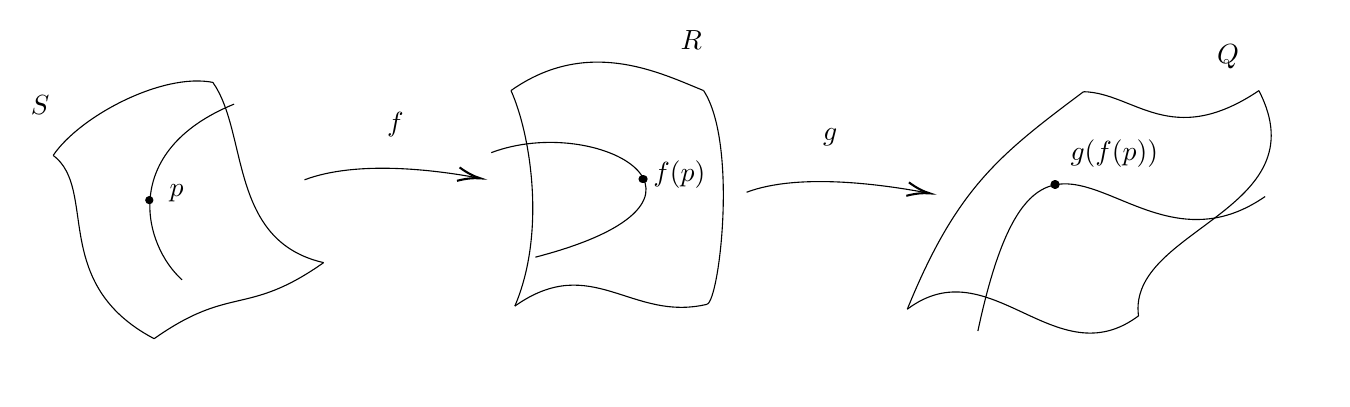
\begin{tikzpicture}[x=0.75pt,y=0.75pt,yscale=-1,xscale=1]
%uncomment if require: \path (0,300); %set diagram left start at 0, and has height of 300

%Curve Lines [id:da029975330356194374] 
\draw    (28.03,88.89) .. controls (40.94,69.88) and (80.84,48.93) .. (104.96,53.73) ;
%Curve Lines [id:da961215863196393] 
\draw    (28.03,88.89) .. controls (49.75,105.22) and (26.09,150.59) .. (76.66,177.21) ;
%Curve Lines [id:da19813598967498913] 
\draw    (104.96,53.73) .. controls (122.13,78.17) and (112.39,130.09) .. (158.32,140.56) ;
%Curve Lines [id:da6872548679722748] 
\draw    (76.66,177.21) .. controls (113.78,151.03) and (121.2,166.74) .. (158.32,140.56) ;
%Curve Lines [id:da20931126567856273] 
\draw    (90.12,148.85) .. controls (71.56,132.27) and (59.5,86.89) .. (115.17,64.2) ;
%Shape: Free Drawing [id:dp43465964553902725] 
\draw  [line width=3] [line join = round][line cap = round] (74.34,110.45) .. controls (74.34,110.45) and (74.34,110.45) .. (74.34,110.45) ;
%Curve Lines [id:da6591471667367296] 
\draw    (149.12,100.67) .. controls (174.39,91.11) and (212.18,95.93) .. (232.14,99.64) ;
\draw [shift={(233.94,99.98)}, rotate = 190.92] [color={rgb, 255:red, 0; green, 0; blue, 0 }  ][line width=0.75]    (10.93,-3.29) .. controls (6.95,-1.4) and (3.31,-0.3) .. (0,0) .. controls (3.31,0.3) and (6.95,1.4) .. (10.93,3.29)   ;
%Curve Lines [id:da047382835709700255] 
\draw    (248.59,57.66) .. controls (257.87,78.17) and (265.76,125.72) .. (250.45,161.5) ;
%Curve Lines [id:da22504090423531187] 
\draw    (248.59,57.66) .. controls (285.71,31.48) and (320.81,49.37) .. (341.38,57.66) ;
%Curve Lines [id:da048314660815029886] 
\draw    (341.38,57.66) .. controls (357.93,82.97) and (349.11,158.45) .. (343.08,160.63) ;
%Curve Lines [id:da43755971494396373] 
\draw    (250.45,161.5) .. controls (287.56,135.32) and (306.43,169.35) .. (343.08,160.63) ;
%Curve Lines [id:da8129727156857004] 
\draw    (239.08,87.58) .. controls (290.5,68.13) and (366.12,110.45) .. (260.34,137.94) ;
%Shape: Free Drawing [id:dp6418697109245284] 
\draw  [line width=3] [line join = round][line cap = round] (312,100.42) .. controls (312.15,100.42) and (312.31,100.42) .. (312.46,100.42) ;
%Curve Lines [id:da5020386509769488] 
\draw    (362.13,106.65) .. controls (387.4,97.1) and (428.45,103.08) .. (448.61,106.86) ;
\draw [shift={(450.42,107.21)}, rotate = 190.92] [color={rgb, 255:red, 0; green, 0; blue, 0 }  ][line width=0.75]    (10.93,-3.29) .. controls (6.95,-1.4) and (3.31,-0.3) .. (0,0) .. controls (3.31,0.3) and (6.95,1.4) .. (10.93,3.29)   ;
%Curve Lines [id:da4733721634332404] 
\draw    (439.54,163) .. controls (463.42,104.21) and (484.42,88.21) .. (524.42,58.21) ;
%Curve Lines [id:da7075571658808304] 
\draw    (524.42,58.21) .. controls (548.92,58.71) and (566.42,86.21) .. (608.92,57.71) ;
%Curve Lines [id:da00793283043838966] 
\draw    (550.92,166.21) .. controls (545.42,124.21) and (638.92,115.71) .. (608.92,57.71) ;
%Curve Lines [id:da3339757498095369] 
\draw    (439.54,163) .. controls (479.54,133) and (510.92,196.21) .. (550.92,166.21) ;
%Curve Lines [id:da3798738761473377] 
\draw    (473.54,173.5) .. controls (503.92,31.21) and (544.92,155.21) .. (611.92,108.71) ;
%Shape: Free Drawing [id:dp98482995655351] 
\draw  [line width=3] [line join = round][line cap = round] (510.5,102.92) .. controls (510.65,102.92) and (510.81,102.92) .. (510.96,102.92) ;

% Text Node
\draw (82.8,101.8) node [anchor=north west][inner sep=0.75pt]    {$p$};
% Text Node
\draw (16,58.6) node [anchor=north west][inner sep=0.75pt]    {$S$};
% Text Node
\draw (187.65,66.89) node [anchor=north west][inner sep=0.75pt]    {$f$};
% Text Node
\draw (315.9,90.02) node [anchor=north west][inner sep=0.75pt]    {$f( p)$};
% Text Node
\draw (329.08,27.63) node [anchor=north west][inner sep=0.75pt]    {$R$};
% Text Node
\draw (397.67,74.87) node [anchor=north west][inner sep=0.75pt]    {$g$};
% Text Node
\draw (516.9,80.02) node [anchor=north west][inner sep=0.75pt]    {$g( f( p))$};
% Text Node
\draw (587.54,34.4) node [anchor=north west][inner sep=0.75pt]    {$Q$};

\end{tikzpicture}
}
\end{center}
